\section{光流法 - Optical Flow}


\subsection{光流法简介}

只有在我们的眼睛(目光)移动的时候,这张图看起来是正在移动!

\begin{figure}
    \centering
    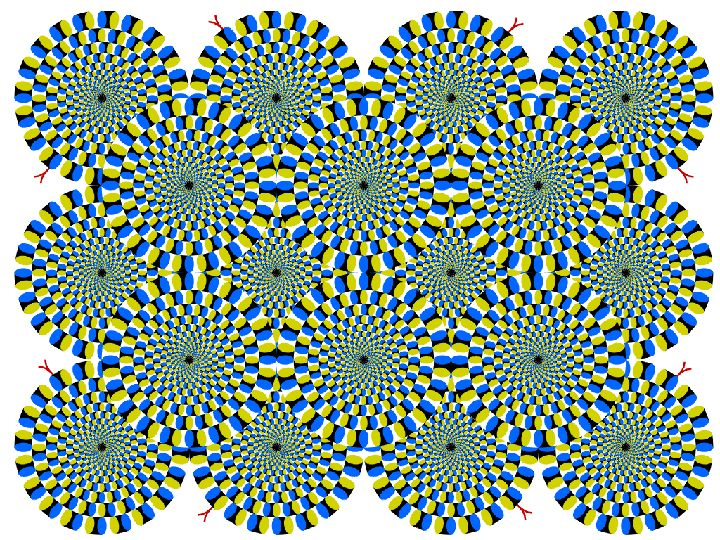
\includegraphics[width=0.5\textwidth]{images/optical_flow_human.jpg}
    \caption{光流}
\end{figure}



\subsection{光流法基本假设}

光流法假设图像具有以下性质

\begin{enumerate}
    \item 在连续的几帧间,目标像素密度不发生变化
    \item 某像素的相邻点和这个像素类似(运动连续)
\end{enumerate}

像素$I(x, y, t)$在$\d t$时间后移动了距离$(\d x, \d y)$,则应有


\begin{equation}
    I(x, y, t) = I(x + \d x, y + \d y, t + \d t)
\end{equation}

因此

\begin{equation}
    \label{eq:optical_flow_eq}
    \frac{\partial I}{\partial x} \frac{\d x}{\d t} + \frac{\partial I}{\partial y} \frac{\d y}{\d t} + \frac{\partial I}{\partial t} = 0
\end{equation}

方程 \refeq{eq:optical_flow_eq} 被称为光流方程(Optical Flow Equation)


\subsection{Lucas-Kanade Method}

Lucas-Kanade方法假设像素点及其周围的8邻域所有的点都满足光流方程。考虑这9个点的两帧之间的关系,我们可以知道$\frac{\partial I}{\partial x}$,$\frac{\partial I}{\partial y}$ 和 $\frac{\partial I}{\partial t}$。我们感兴趣的量是$(\frac{\d x}{\d t}, \frac{\d y}{\d t})$的值,可以用最小二乘法求得,即有

\begin{equation}
    \begin{bmatrix}
        \frac{\d x}{\d t} \\
        \frac{\d y}{\d t}
    \end{bmatrix} = \begin{bmatrix}
        \sum f_x^2   & \sum f_x f_y \\
        \sum f_x f_y & \sum f_y^2   \\
    \end{bmatrix}^{-1} \begin{bmatrix}
        -\sum f_x f_t \\
        -\sum f_y f_t \\
    \end{bmatrix}
\end{equation}